\documentclass[xcolor=dvipsnames]{beamer}

%%% Packages %%%
\usepackage{graphicx}
\usepackage[utf8]{inputenc}
\usepackage{subfig}
\usepackage{tikz}
\usepackage[absolute, overlay]{textpos}
\usepackage{soul}
\usepackage{booktabs}
\usepackage{multicol}
\usepackage{multimedia} % For movies
\usepackage{pgfplots} % For generating random numbers for tikz 
\usepackage{pstricks-add}
\usepackage{comment}

\usetikzlibrary{calc}
\usetikzlibrary{shapes.geometric}
\usetikzlibrary{arrows}

%%% Creating Tarleton Purple %%%
\definecolor{TarletonPurple}{RGB}{79, 45, 127}
\definecolor{ufsdxf}{rgb}{0.30980392156862746,0.17647058823529413,0.4980392156862745}


%%% Beamer Theme %%%
\usetheme{Copenhagen}
\usecolortheme[named=TarletonPurple]{structure}


%%% Graphics Path %%%
\graphicspath{{./images}}

%%% Title Page Info %%%
\title{SYNC or Swim}
\subtitle{A Particle Model of the Interaction within Fish Schools}
\author{David Ebert and Mikaela Jordan}
\institute{Tarleton State University}
\date{March 31, 2017}

%%% Making Reference Environment For Tarleton Picture %%%
\newenvironment{reference}[2]{
\begin{textblock*}{\textwidth}(#1,#2)              
  \footnotesize\it\bgroup\color{red!50!black}}{\egroup\end{textblock*}}

%%% Setting node styles for isosceles triangles %%%
\tikzset{
	focal/.style={
		draw=Magenta,
		shape=isosceles triangle,
		fill=Magenta!30,
		shape border uses incircle,
		minimum height= 0.15cm, 
		minimum width= 0.1cm,
		shape border rotate=#1,
		isosceles triangle stretches,
		inner sep=0pt
	},
	focalfish/.style={focal=+90}
}

\tikzset{
	fish/.style={
		draw=MidnightBlue,
		shape=isosceles triangle,
		fill=MidnightBlue!50,
		minimum height= 0.15cm, 
		minimum width= 0.1cm,
		shape border rotate=90,
		isosceles triangle stretches,
		inner sep=0pt
	}
}

%%% The document %%%
\begin{document}
\makeatletter
\def\beamer@framenotesbegin{
\begin{reference}{107mm}{0.5mm}
\tikz\node[opacity=1.0]{
\includegraphics[scale=0.4]{images/tsumath_copy}};
\end{reference} 
}

\frame{\titlepage}

\begin{frame}
	\frametitle{Synchronization}
	The coordination of events to operate a system in unison.\\ 
	Some examples:
	\begin{itemize}
		\item Circadian Rhythms
	\end{itemize}
	\vspace{100 pt}
\end{frame}

\begin{frame}
	\frametitle{Synchronization}
	The coordination of events to operate a system in unison.\\ 
	Some examples:
	\begin{itemize}
		\item Animal Swarming 
	\end{itemize}
	\begin{center}
	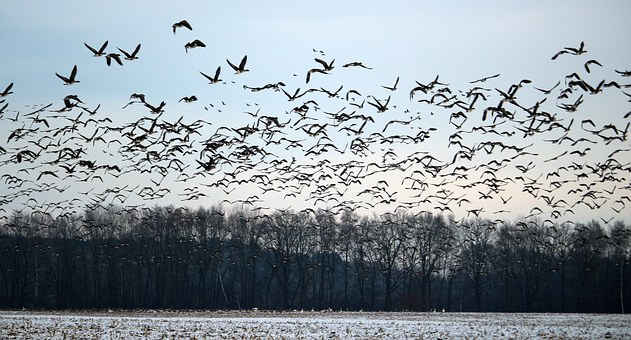
\includegraphics[scale=1.15]{images/geese_flock.jpg}
	\end{center}
	\vspace{5 pt}
\end{frame}

\begin{frame}
	\frametitle{Synchronization}
	The coordination of events to operate a system in unison.\\ 
	Some examples:
	\begin{itemize}
		\item Human Imitation (Memes/Trends) 
	\end{itemize}
	\begin{center}
	
\includegraphics[scale=0.15]{images/salt_guy.jpg}
	\end{center}
\end{frame}

\begin{frame}
	\frametitle{Synchronization}
	The coordination of events to operate a system in unison.\\ 
	Some examples:
	\begin{itemize}
		\item Round of Applause
	\end{itemize}
	\vspace{100 pt}
\end{frame}


\begin{frame}
	\frametitle{Example}
\noindent Rules to Follow:
\begin{itemize}
	\item \textbf{Walk} slowly toward center of the group.
	\item \textbf{Slow down} if you're within two feet of another person.
	\item \textbf{Stop} if you are within one foot of another person.
\end{itemize}

% The movie won't play in a normal .pdf viewer. Okular works.
\centering
\movie[width=5cm,height=4cm, poster, showcontrols]{}{human_swarm.ogv} 
\end{frame}


\begin{frame}
	\frametitle{Collective Behavior}
	\begin{center}
	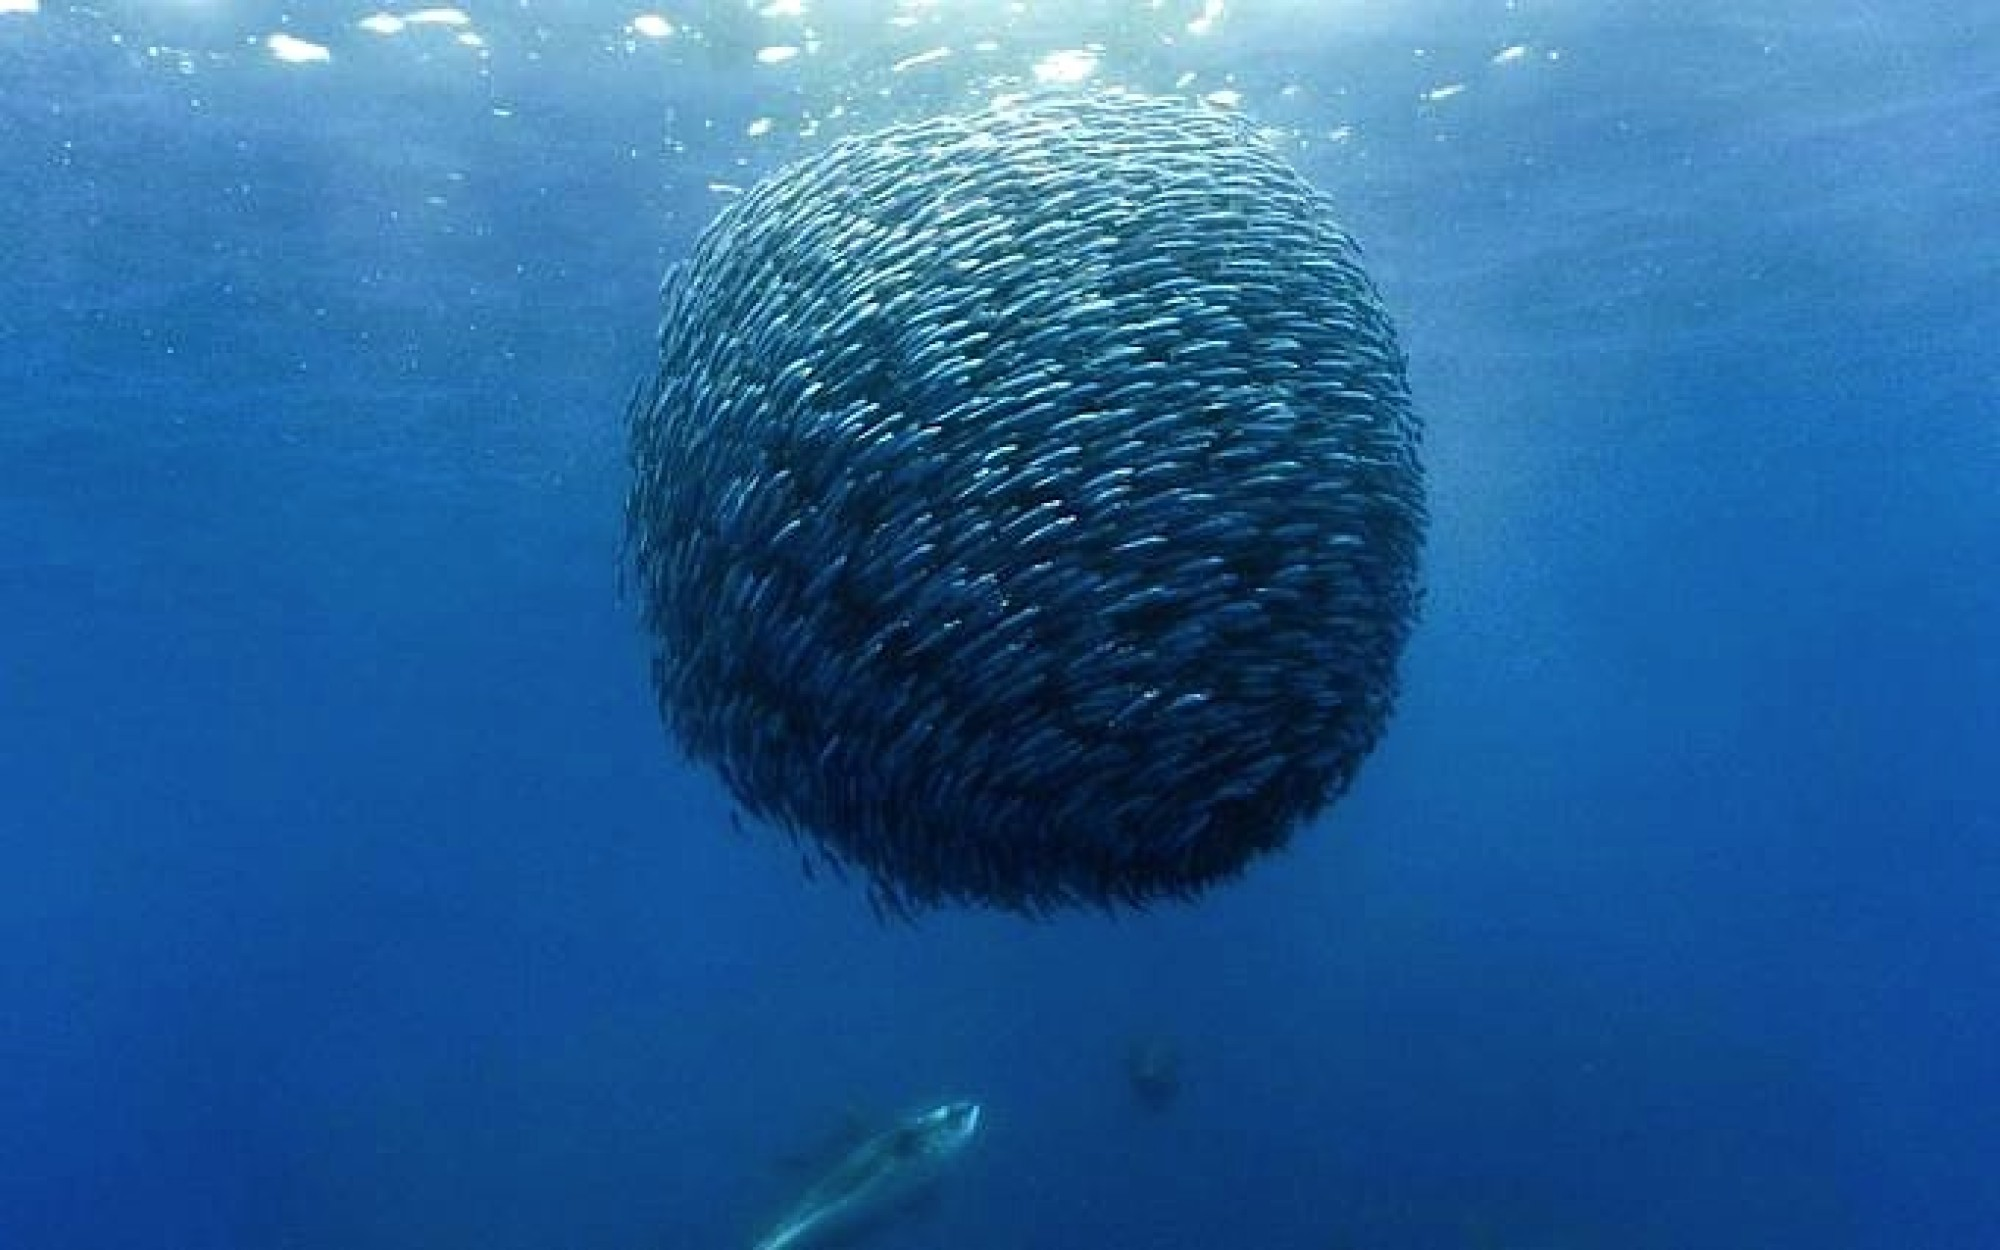
\includegraphics[scale=0.05]{images/fish_schoo.jpg}
	\end{center}
	\begin{itemize}
		\item The coordinated behavior of animals of the same species and the emergent properties that arise.
		\pause
		\item For mathematical purposes, consider a swarm as an emergent behavior with no central coordination.
	\end{itemize}
\end{frame}

\begin{frame}
	\frametitle{Why Do We Care?}
	\begin{itemize}
		\item Learning C, CUDA, OpenGL, modeling
		\item How will environmental factors affect the animal aggregate?
		\item How will animal aggregates affect the environment?
	\end{itemize}
\end{frame}

\begin{frame}
	\frametitle{Schooling Model}
	\begin{multicols}{2}
	\onslide<1->{
	Our model represents each fish adhering to the following three rules:}
	\begin{itemize}
		\onslide<2->{
			\item \textbf{Alignment}}
		\onslide<3->{
			\item \textbf{Cohesion}} 
		\onslide<4->{
			\item \textbf{Separation}}
%		Avoid collisions with neighbors
	\end{itemize}
	\begin{figure}
		\centering
		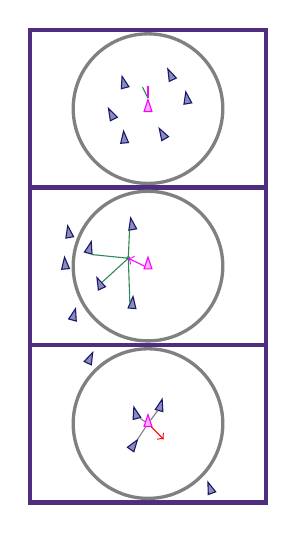
\begin{tikzpicture}
			\onslide<2>{
				\draw[ultra thick, TarletonPurple] (0, 4) rectangle (3, 6);
				\draw[very thick, gray] (1.5, 5) circle [radius=0.95cm];
				%%% Alignment %%%
				
				\node[focalfish] (focal1) at (1.5, 5) {};
				\node[fish, rotate=15] (align1) at ($(focal1) + (-0.3, 0.3)$) {};
				\node[fish, rotate=25] (align2) at ($(focal1) + (0.3, 0.4)$) {};
				\node[fish, rotate=10] (align3) at ($(focal1) + (0.5, 0.1)$) {};
				\node[fish, rotate=30] (align4) at ($(focal1) + (0.2, -0.35)$) {};
				\node[fish, rotate=5] (align5) at ($(focal1) + (-0.3, -0.4)$) {};
				\node[fish, rotate=27] (align6) at ($(focal1) + (-0.45, -0.1)$) {};
				
				\draw[Magenta] (focal1.north) -- ($(focal1.north) + (0, 0.15)$);
				\draw[SeaGreen] (focal1.north) -- ($(focal1.north) + (-0.07, 0.14)$);
			}
			
			\onslide<3>{
				\draw[ultra thick, TarletonPurple] (0, 2) rectangle (3, 4);
				\draw[very thick, gray] (1.5, 3) circle [radius=0.95cm];
				%%% Cohesion %%%
				\node[focalfish] (focal2) at (1.5, 3) {};
				\node[fish, rotate=10] (coh1) at ($(focal2) + (-0.2, 0.5)$) {};
				\node[fish, rotate=-15] (coh2) at ($(focal2) + (-0.75, 0.2)$) {};
				\node[fish, rotate=25] (coh3) at ($(focal2) + (-0.6, -0.25)$) {};
				\node[fish, rotate=-5] (coh4) at ($(focal2) + (-0.2, -0.5)$) {};
				\node[fish, rotate=10] (coh5) at ($(focal2) + (-1, 0.4)$) {};
				\node[fish, rotate=5] (coh6) at ($(focal2) + (-1.05, 0)$) {};
				\node[fish, rotate=-15] (coh7) at ($(focal2) + (-0.95, -0.65)$) {};
				
				\draw[SeaGreen] (coh1.south west) -- (1.25, 3.1);
				\draw[SeaGreen] (coh2.south east) -- (1.25, 3.1);
				\draw[SeaGreen] (coh3.north east) -- (1.25, 3.1);
				\draw[SeaGreen] (coh4.north west) -- (1.25, 3.1);
				
				\fill[SeaGreen] (1.25, 3.1) circle [radius=0.75pt];
				
				\draw[Magenta, ->] (focal2.west) -- (1.25, 3.1);
				}
				
			\onslide<4>{
				\draw[ultra thick, TarletonPurple] (0, 0) rectangle (3, 2);
				\draw[very thick, gray] (1.5, 1) circle [radius=0.95cm];
				%%% Separation %%%
				\node[focalfish] (focal) at (1.5, 1) {};
				\node[fish, rotate=15] (fish1) at ($(focal) + (-0.15, 0.1)$)  {};
				\node[fish, rotate=-15] (fish2) at ($(focal) + (0.15, 0.2)$) {};
				\node[fish, rotate=-35] (fish3) at ($(focal) + (-0.2, -0.3)$) {};
				\node[fish, rotate=20] (fish4) at ($(focal) + (0.8, -0.85)$) {};
				\node[fish, rotate=-25] (fish5) at ($(focal) + (-0.75, 0.8)$) {};
			
				\draw[thin, gray] (focal) -- (fish1);
				\draw[thin, gray] (focal) -- (fish2);
				\draw[thin, gray] (focal) -- (fish3);
			
				\draw[red, ->] (focal) -- ($(focal) + (0.2, -0.2)$);}
			
		
		\end{tikzpicture}
	\end{figure}
	\end{multicols}
\end{frame}

\begin{frame}
	\frametitle{The Mathematics}
	\begin{itemize}
		\onslide<1>{
		\item Lagrangian Algorithm}
		\onslide<2->{
		\item Metric distance model}
	\end{itemize}
	\begin{figure}
		\centering
		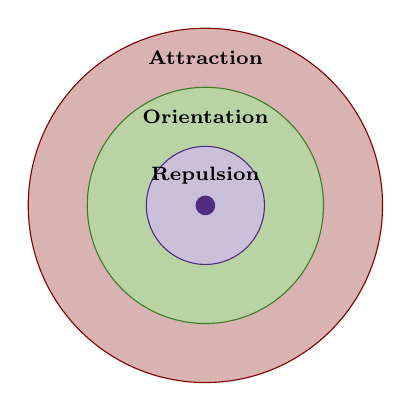
\begin{tikzpicture}[scale=0.5]
			\onslide<5->{
			\filldraw[fill=Maroon!30, draw=Maroon] (0, 0) circle [radius=4.5cm];}
			\onslide<4->{
			\filldraw[fill=OliveGreen!30, draw=OliveGreen] (0, 0) circle [radius=3cm];}
			\onslide<3->{
			\filldraw[fill=TarletonPurple!30, draw=TarletonPurple] (0, 0) circle [radius=1.5cm];}
			\onslide<3->{
			\fill[TarletonPurple] (0, 0) circle [radius=0.25cm];}
			
			\onslide<5->{
			\node at (0, 3.75) {\scriptsize{\textbf{Attraction}}};}
			\onslide<4->{
			\node at (0, 2.25) {\scriptsize{\textbf{Orientation}}};}
			\onslide<3->{
			\node at (0, 0.75) {\scriptsize{\textbf{Repulsion}}};}
		\end{tikzpicture}
	\end{figure}
\end{frame}


\begin{frame}
	\frametitle{Attractive and Repulsive Forces Between Fish}
	\begin{itemize}
		\onslide<1>{
		\item Attraction between a fish $i$ and neighbor $j$ :}
			\onslide<1->{
			\begin{equation*}
				\textcolor{Maroon}{A = C_{a} \frac{p_{j} - p_{i}}{d^{2}}}
			\end{equation*}}
		\onslide<2>{
		\item Repulsion between fish $i$ and neighbor $j$:}
			\onslide<2->{
			\begin{equation*}
				\textcolor{TarletonPurple}{R = -C_{r} \frac{p_{j} - p_{i}}{d^{4}}}	
			\end{equation*}}
		\onslide<3>{
		\item Overall Attraction:
			\begin{equation*}
				F_{A} = \textcolor{Maroon}{C_{a} \frac{p_{j} - p_{i}}{d^{2}}} \textcolor{TarletonPurple}{- C_{r} \frac{p_{j} - p_{i}}{d^{4}}}
			\end{equation*}}

	\end{itemize}
\end{frame}


\begin{comment}
\begin{frame}
	\frametitle{The Attraction and Repulsion Coefficients}
	\begin{equation*}
	f(x) = \frac{2}{x^{2}} - \frac{1}{x^{4}}
	\end{equation*}
	\begin{figure}
		\centering
<<<<<<< HEAD
%		\includegraphics[scale=0.5]{images/coefficient_plot.png}
		\psset{xunit=0.5cm,yunit=0.5cm,algebraic=true,dimen=middle,dotstyle=o,dotsize=5pt 0,linewidth=0.8pt,arrowsize=3pt 2,arrowinset=0.25}
		\begin{pspicture*}(0.,-2.8631891087147996)(6.5648188315047395,4.8322794702689515)
			\psaxes[labelFontSize=\scriptstyle,xAxis=true,yAxis=true,Dx=1.,Dy=1.,ticksize=-2pt 0,subticks=2]{->}(0,0)(0.,-2.8631891087147996)(6.5648188315047395,4.8322794702689515)
			\onslide<2->{
			  \psplot[linewidth=1.2pt,linecolor=ufsdxf,plotpoints=200]{6.56481883150474E-6}{6.5648188315047395}{-1.0/x^(4.0)+2.0/x^(2.0)}
			}
			\begin{scriptsize}
				\onslide<2->{
				  \rput[bl](-7.819787819980308,-0.14017714999747297){\ufsdxf{$f$}}
				}
			\end{scriptsize}
		\end{pspicture*}
=======
		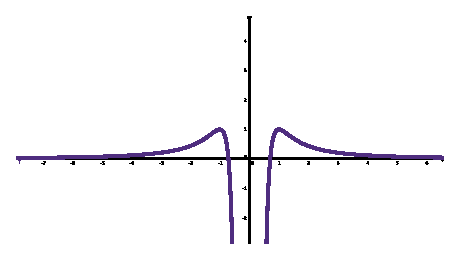
\includegraphics[scale=1]{images/coeff_plot2}
<<<<<<< HEAD
		\begin{tikzpicture}
			\begin{axis}[
				axis lines = left,
				xlabel = {Distance},
				ylabel = {Attraction},
				xmin = 0,
				xmax = 10,
				ymin = -10,
				ymax = 10
			]
			\addplot[
				domain=0.1:10,
				samples=100,
				color=TarletonPurple
			]
			{(2/(x^{2}) - (1/x^{4})}
			\addlegendentry{\frac{2}{x^{2}} - \frac{1}{x^4}}}
			\end{axis}
		\end{tikzpicture}
=======
%		\begin{tikzpicture}
%			\begin{axis}[
%				axis lines = left,
%				xlabel = {Distance},
%				ylabel = {Attraction},
%				xmin = 0,
%				xmax = 10,
%				ymin = -10,
%				ymax = 10
%			]
%			\addplot[
%				domain=0.1:10,
%				samples=100,
%				color=TarletonPurple
%			]
%			{(2/(x^{2}) - (1/x^{4})}
%			\addlegendentry{\frac{2}{x^{2}} - \frac{1}{x^4}}}
%			\end{axis}
%		\end{tikzpicture}
>>>>>>> 8ebfde8f337e70cee5bc542ce49aad7a09dd5b3d
>>>>>>> c38eeb5ab0bd8f7f9015db53a9c83f2d79ef2541
	\end{figure}
\end{frame}
\end{comment}

\begin{frame}
	\frametitle{Directional Alignment of Fish $i$}
	\begin{multicols}{2}
	\begin{figure}
		\centering
		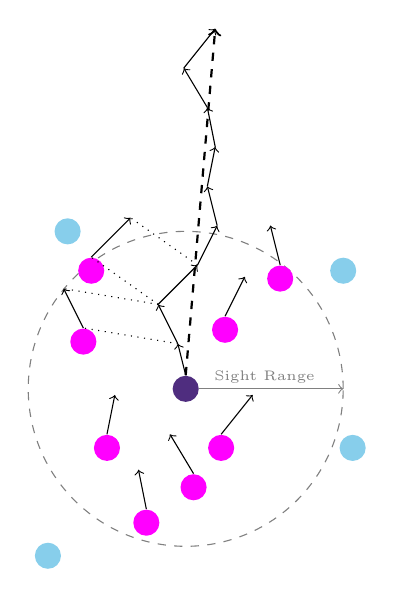
\begin{tikzpicture}[focalfish/.style={circle, minimum size=1mm, fill=TarletonPurple}, fish/.style={circle, minimum size=1mm,
			fill=Magenta}, outfish/.style={circle, minimum size=1mm, fill=SkyBlue}]
			\draw[dashed, gray] (0, 0) circle [radius=2cm];
			
			\node[focalfish] (focal) at (0, 0) {};
			\draw[->] (focal.north) -- ($(focal.north) + (-0.1, 0.4)$);
			
			%%% Radius Vector %%%
			\draw[gray, ->] (focal.east) -- (0:2cm);
			\node at (1, 0.15) {\tiny{\textcolor{gray}{Sight Range}}};
			
			
			\node[fish] (infish1) at (0.5, 0.75) {};
			\node[fish] (infish2) at (1.2, 1.4) {};
			\node[fish] (infish3) at (-1.2, 1.5) {};
			\node[fish] (infish4) at (-1.3, 0.6) {};
			\node[fish] (infish5) at (-1, -0.75) {};
			\node[fish] (infish6) at (-0.5, -1.7) {};
			\node[fish] (infish7) at (0.1, -1.25) {};
			\node[fish] (infish8) at (0.45, -0.75) {};
			\node[outfish] (fish9) at (-1.5, 2) {};
			\node[outfish] (fish10) at (-1.75, -2.12) {};
			\node[outfish] (fish11) at (2, 1.5) {};
			\node[outfish] (fish12) at (2.12, -.75) {};
%			\node[fish] (fish13) at (0.5, 0.75) {13};
%			\node[fish] (fish14) at (0.5, 0.75) {14};
			
			\draw[->] (infish1.north) -- ($(infish1.north) + (0.25, 0.5)$);
			\draw[->] (infish2.north) -- ($(infish2.north) + (-0.125, 0.5)$);
			\draw[->] (infish3.north) -- ($(infish3.north) + (0.5, 0.5)$);
			\draw[->] (infish4.north) -- ($(infish4.north) + (-0.25, 0.5)$);
			\draw[->] (infish5.north) -- ($(infish5.north) + (0.1, 0.5)$);
			\draw[->] (infish6.north) -- ($(infish6.north) + (-0.1, 0.5)$);
			\draw[->] (infish7.north) -- ($(infish7.north) + (-0.3, 0.5)$);
			\draw[->] (infish8.north) -- ($(infish8.north) + (0.4, 0.5)$);
			
			\onslide<2-4>{
			\draw[dotted,] ($(focal.north) + (-0.1, 0.4)$) -- (infish4.north);
			\draw[->] ($(focal.north) +(-0.1, 0.4)$) -- ($(focal.north) +(-0.1, 0.4) + (-0.25, .5)$);
			\draw[dotted] ($(focal.north) +(-0.1, 0.4) + (-0.25, .5)$) -- ($(infish4.north) + (-0.25, 0.5)$);}
			\onslide<3-4>{
			\draw[dotted] ($(focal.north) +(-0.35, 0.9)$) -- (infish3.north);
			\draw[->] ($(focal.north) + (-0.35, 0.9)$) -- ($(focal.north) + (-0.35, 0.9) + (0.5, 0.5)$);
			\draw[dotted] ($(focal.north) + (0.15, 1.4)$) -- ($(infish3.north) + (0.5, 0.5)$);}
			\onslide<4>{
			\draw[->] ($(focal.north) + (0.15, 1.4)$) --  ($(focal.north) + (0.15, 1.4) + (0.25, 0.5)$);
			\draw[->] ($(focal.north) + (0.4, 1.9)$) -- ($(focal.north) + (0.4, 1.9) + (-0.125, 0.5)$);
			\draw[->] ($(focal.north) + (0.275, 2.4)$) -- ($(focal.north) + (0.275, 2.4) + (0.1, 0.5)$);
			\draw[->] ($(focal.north) + (0.375, 2.9)$) -- ($(focal.north) + (0.375, 2.9) + (-0.1, 0.5)$);
			\draw[->] ($(focal.north) + (0.275, 3.4)$) -- ($(focal.north) +  (0.275, 3.4) + (-0.3, 0.5)$);
			\draw[->] ($(focal.north) + (-0.025, 3.9)$) -- ($(focal.north) + (-0.025, 3.9) + (0.4, 0.5)$);}
			
			\onslide<5->{
			\draw[->, thick, dashed] (focal.north) -- ($(focal.north) + (0.375, 4.4)$);}
		\end{tikzpicture}
	\end{figure}
	\onslide<6->{
	\begin{equation*}
		F_{D_i} = \textcolor{OliveGreen}{\sum\limits_{j=1}^{N}\frac{v_{j}}{|| p_{i} - p_{j}||}}
	\end{equation*}}
	\end{multicols}
\end{frame}

\begin{frame}
	\frametitle{Total Force on Fish $i$ From All Neighbors}
	\begin{equation}
		F_{i_N} = \sum\limits_{j=1}^{N}\bigg( W_{a}\big( \textcolor{Maroon}{C_{a}\frac{p_{j} - p_{i}}{d^{2}}} \textcolor{TarletonPurple}{- C_{r}\frac{p_{j} - p_{i}}{d^{4}}} \big) + W_{d} \big(\textcolor{OliveGreen}{\frac{v_{j}}{||p_{i} - p_{j}||}\big) \bigg)}
	\end{equation}
	\pause 
	And, acceleration of each fish is the same as our force (taking each mass to be 1).
\end{frame}

\begin{frame}
	\frametitle{Calculating Forces, Velocities, and Positions}
	At every timestep, the following calculations occur for each particle (let's call it particle $i$):
	\begin{enumerate}
		\onslide<2>{
		\item Calculate $||p_{i} - p_{j}||$}.
		\onslide<3>{
		\item If the $||p_{i} - p_{j}|| <$ SIGHT, use (1) to determine the force between particle $j$ and particle $i$, and sum forces over all particles within SIGHT of particle $i$ ($F_{i_N}$).}
		\onslide<4>{
		\item Use $F_{i_N}$ calculated above to update particle $i$'s velocity as follows:
			\begin{equation*}
				v_{i} = v_i + F_{i_N}\cdot dt
			\end{equation*}}
		\onslide<5>{
		\item And update particle $i$'s position using: 
			\begin{equation*}
				p_{i} = p_{i} + v_{i}\cdot dt	
			\end{equation*}}

		
	\end{enumerate}
\end{frame}

\begin{frame}{Simulations}
	\begin{center}
		% The movie won't play in a normal .pdf viewer. Okular works.
		\movie[width=7.0cm,height=7.0cm, poster, showcontrols]{}{2D_coalesce.ogv}
	\end{center}
\end{frame}

\begin{frame}{Simulations}
	\begin{center}
		% The movie won't play in a normal .pdf viewer. Okular works.
		\movie[width=7.0cm,height=7.0cm, poster, showcontrols]{}{2D_predator.ogv}
	\end{center}
\end{frame}

\begin{frame}{Simulations}
	\begin{center}
		% The movie won't play in a normal .pdf viewer. Okular works.
		\movie[width=7.0cm,height=7.0cm, poster, showcontrols]{}{3D_movie.ogv}
	\end{center}
\end{frame}

\begin{frame}
	\frametitle{Where Do We Go From Here?}
	\begin{itemize}
		\item Add initial conditions for species-specific parameters 
			\begin{itemize}
				\item Density of swarms, how they behave towards targets and obstacles, etc.
			\end{itemize}
		\item Move calculations from CPU to GPU to speed up calculation time
	\end{itemize}
\end{frame}

\begin{frame}
	\frametitle{References}
	\footnotesize{
	Barbaro, Alethea, Bjorn Birnir, and Kirk Taylor. \textit{Simulating the Collective} \\
	\hspace{0.5cm} \textit{Behavior of Schooling Fish With a Discrete Stochastic Model}. University\\
	\hspace{0.5cm} of Iceland. 2006. Web. \\
	
	\noindent Bernoff, Andrew J. ``Synchronization and Swarming: Clocks and Flocks.'' \\
	\hspace{0.5cm} Harvey Mudd College. \\
	
	\noindent Morale, Daniela, Vincenzo Capasso, and Karl Oelschlager.``An Interacting \\
	\hspace{0.5cm} Particle System Modelling Aggregation Behavior: From Individuals to\\
	\hspace{0.5cm} Populations''. \textit{Journal of Mathematical Biology}. 2004. Web.
	
	\noindent Parrish, Julia K., Steven V. Viscido, and Daniel Grunbaum. ``Self-Organized \\
	\hspace{0.5cm} Fish Schools: An Examination of Emergent Properties''. \\  
	\hspace{0.5cm} \textit{The Biological Bulletin} 202. 2002:296-305. Web. \\
	
	\noindent Schellinck, Jen, and Tony White. ``A Review of Attraction and Repulsion\\
	\hspace{0.5cm} Models of Aggregation: Methods, Findings, and a Discussion of Model \\
	\hspace{0.5cm} Validation''. \textit{Ecological Modelling} 222. 2011: 1897-1911. Web.
	}
\end{frame}

\begin{frame}
	\frametitle{THANK YOU} 
	Thank you to Dr. Wyatt and the Particle Modelling Lab for their time and resources.
	\vspace{20 pt}
	\begin{center}
		{\Huge QUESTIONS?} \\
	\end{center}
	\vspace{20 pt}	
	%\textbf{Contact:} \\
	\texttt{mikaela.jordan@go.tarleton.edu} \\
	\texttt{david.ebert@go.tarleton.edu} \\
	\texttt{github.com/dpebert7/sync} \\
\end{frame}

\end{document}
